\chapter{Related work} 

\chapterintro{This chapter presents recent achievements in a field of platform-as-a-service model by examining: Carina, OneFlow, CloudFoundry and OpenShift. Especially, it focuses on aspects of adaptivity, scalability and cloud federation awareness.}

\section{Requirements}
One can notice that elements that yields a solution to a problem stated in the first chapter, which is ensuring that users' application provide appropriate Quality-of-Service for its customers in a most-cost effective manner, were gradually introduced in previous chapters:

\begin{itemize}
	\item \emph{adaptivity} - ability to adapt (i.e. scale) appropriately to a current usage pattern
	\item \emph{scalability} - ability to improve application performance by enriching resources
	\item \emph{cloud-federation awareness} - ability to compose an application deployment using different cloud providers; cooperation with different cloud provider to supply application with extra resources while performing application scaling
\end{itemize}

Next section states the general overview of the proposed solution, while the consecutive sections details its elements and finally the last section summarises the design choices in a context of system requirements.
	
% radek
\section{Carina}

\subsection{Introduction}
Carina is an open source project, released under Apache License 2.0, built on top of OpenNebula, which aims to ``(\ldots) standardize the process for automating multi-VM deployments and setting auto-scaling and availability management policies in the cloud.'' \cite{CarinaBlog}. The project is used by the authors at their work at RIM in an OpenNebula-based private cloud.

\subsection{Features}
As it is stated in the requirements of the solution, \emph{Carina} should support variety of features which can be considered worth scrutinizing carefully as they are closely related to notions of adaptivity and scalability. To name the most relevant: \cite{CarinaBlog}
\begin{itemize}
  \item Collect and aggregate OS or app-specific metrics across a cluster
  \item Drive elastic scaling of clusters based on workload or events
  \item Support deployment and handling of failover of services across multiple datacenters
\end{itemize}

Before delving into more detailed description it is vital to introduce most important terms used in \emph{Carina} documentation to depict this product:
\begin{itemize}
  \item Environment -- a collection of VMs in a master-slave configuration,
  \item Service -- a consumer of cloud resources. Each service can have its own environment configurations and create environments and control them independently of other services,
  \item Pools -- various clusters or virtual data centers in OpenNebula that can be targets for creating an environment
\end{itemize}

\subsection{Key technical concepts}

\subsubsection{Adaptivity}
In \emph{Carina} there are mechanisms which can perform application scaling, both in manual and automatic fashion. It is possible for a system administrator to directly modify the existing application and its environment by changing its parameters manually. Automatic management of an environment is done by defining \emph{scaling policies} which can be in two flavours: \emph{time-based} and \emph{load-based}. Those are called by the authors \emph{elasticy policies}.

\emph{Time-based} policies defines how the system should react in the given window frame(s). In each frame we can specify the minimum number of virtual machines that comprises an environment. On the other hand, \emph{load-based} policies define the way the system reacts to \textbf{average cpu usage} by the environment. This is the simplest \emph{threshold-model} as introduced in chapter 2. The user enters predicates which are evaluated against data gathered by OpenNebula and execute scaling actions  (\emph{scaleup} and \emph{scaledown}) if they are true. What is more, the minimal and maximal number of virtual machines must be specified. At present the only parameter that is taken into account while performing actions triggered by \emph{load-based} policies is cpu usage.

To increase the application availability, \emph{Carina} introduces the notion of \emph{availability policies}. Their main function is to take a recovery action in response to a deletion or errors during deployment of a virtual machine. Recreation of a virtual machine is the most fundamental and atomic operation under this model.

\subsubsection{Scaling}
Chapter 3 introduced and discussed various types of application scaling. \emph{Carina} offers only one type of scaling and this is \emph{horizontal} scaling -- user's capabilities are limited only to add/remove a virtual machine to/from a given environment. Unfortunately there are no means to modify the parameters of a given or a set of virtual machines.

\subsubsection{Cloud federation awareness}
In this paper we strongly advocate spanning cloud resources across multiple vendors/providers. Despite having in its requirements such a position, \emph{Carina} \textbf{does not} support deployment or scaling of services across different providers. In the environment configuration we define only \textbf{one} endpoint -- this is can be thought of a reference to a cloud provider. As it can be only one per environment, it is not possible to deploy or scale some artifacts across many providers.

\subsection{Design}
To complete the discussion about \emph{Carina} it is essential to include its architecture overview. This is shown in figure \ref{sota:carina-design}.

\begin{figure}[!ht]
  \begin{center}
    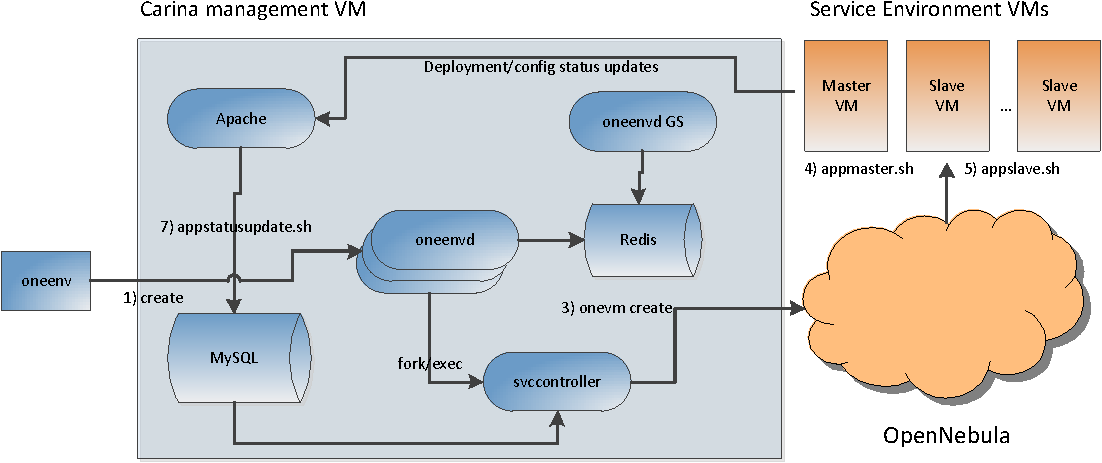
\includegraphics[width=\textwidth]{chapter-state-of-the-art/carina-design}
  \end{center}
  \caption{Carina -- components interaction}
  \label{sota:carina-design}
\end{figure}

There are number of things that cause concern:
\begin{asparaenum}
\item[\textbf{Persistency}] No one knows for what reason, but \emph{Carina} uses two databases. What makes things even worse, they completely differ in types, as \emph{MySQL} is a relational and \emph{redis} is a nosql database. This places additional burden on technical requirements of the platform.
\item[\textbf{Usage of Apache}] To work properly, \emph{Carina} needs Apache http server. In the server cgi-bin directory there are placed bash scripts which are invoked by contextualization scripts executed in different stages of virtual machines life cycle. Instead, we recommend setting proper web services, environment-agnostic, in a central node which can be run next to global scheduler.
\item[\textbf{User accounts}] \emph{Carina} forces the creation of a system-wide user for each service. These concepts should be totally independent.
\item[\textbf{Provisioning}] User has to use in the environment specification previously defined OpenNebula images. Their further adjusting happens in the contextualization phase. This forces the user to modify the state of a virtual machine when there is a need to perform any changes, for example in the software stack. Instead we suggest using some provisioning software such as puppet or chef -- this would enable users to change software stack only in configuration files (recipes) not by altering the virtual machine state.
\end{asparaenum}

\subsection{Summary}
\emph{Carina} emerged as a promising platform built on top of OpenNebula, which lacked most of its functionalities at that time. The good point is the fact that this product is used in a business context and judging by the authors' description it actually works. However, due to deficiencies mentioned in the previous sections, \emph{Carina} cannot be considered a mature and generic solution for more demanding cloud providers.



\section{OneFlow}

\subsection{Introduction}
\emph{OneFlow} \cite{OneFlow} is a management system integrated into \emph{OpenNebula} that aspires to enhance it with multi-tiered applications (service) deployment and auto-scaling capabilities. It is available as a core part of \emph{OpenNebula} since 4.2 version and released under \emph{Apache License, Version 2.0}. 

\subsection{Features}
In a context of this thesis, \emph{OneFlow} enriches \emph{OpenNebula} with only one, yet powerful feature: application scaling based on policies. Besides this, benefits of using \emph{OneFlow} are as follows:
\begin{itemize}
\item defining multi-tiered applications (services) as a collection of applications
\item providing configurable services from a catalogue and self-service portal
\item enabling tight, efficient administrative control
\item fine-grained access control for the secure sharing of services with other users
\end{itemize}

\subsection{Key technical concepts}
\subsubsection{Adaptivity}
Adaptivity is achieved by specifying policies, that violated, trigger events impacting service environment. There are two types of policies available:
\begin{itemize}
 \item \emph{Auto-scaling based on metrics} - policy defines an expression that triggers scaling adjustments. Expressions can use performance data sent from virtual machine using \emph{OneGate} as well as virtual machine data such as CPU, memory, network bandwidth
 \item \emph{Auto-scaling based on schedule} - policy specifies a time or a time recurrence and correlates that information to appropriate service adjustments
\end{itemize}

Apart from scaling policies, scaling is controlled by a minimal and maximal number of virtual machines that can compose a service.

\subsubsection{Scaling}
\emph{OneFlow} is capable of \textbf{only} horizontal scaling: it adds or removes virtual machine using \emph{OpenNebula API}, when appropriate event is triggered. Violating given policy results in virtual machine's state transition into \texttt{SCALING}. After proper action is finished, virtual machines converges to a \texttt{COOLDOWN} state. What this simple state transition does is allows an environment to accommodate changes and adjust to a recent changes, disabling scaling for a given period of time.


\subsubsection{Cloud federation awareness}
\emph{OneFlow} itself \textbf{does not} cooperate with different cloud instance. Hence, one is limited to \emph{OpenNebula} hybrid or public cloud capabilities that employs oZones and \emph{AWS}, respectively. Although, they expand single \emph{OpenNebula} instance capacity it is limited in a way that discriminates it as possible solution. Firstly, the problem with oZones is that they require centralised management, while cloud federation is by definition distributed and independent. Secondly, cloud bursting into \emph{AWS} limits instance monitoring capabilities. Consequently, it is not possible to supervise provisioned instances.

\subsection{Summary}
Taking everything into consideration, OneFlow is a valuable addition to OpenNebula ecosystem. Undoubtedly, its auto-scaling feature with elastic policy mechanism cannot be underestimated. However, actions taken by scaling mechanism are coarse-grained by being limited to a horizontal scaling. What makes things worse, OneFlow can not leverage resources of multiple providers associated within a cloud federation.

\section{OpenShift}

\subsection{Introduction}
\emph{OpenShift} is developed by \emph{RedHat} Platform-as-a-Service solution. It is available in two different flavours:
\begin{itemize}
 \item \emph{OpenShift Enterprise} (private cloud)
 \item \emph{OpenShift Online / FreeShift} hosted by RedHat (public cloud)
\end{itemize}

The latter is freely distributed, but it is limited to only 3 gears (a 'gear' is a resource maintained by \emph{OpenShift}, such as application server or database). Beside this, source code is hosted on github and licensed under \emph{Apache License 2.0}.

\subsection{Features}
High level features that distinguishes \emph{OpenShift} are as follows:
\begin{itemize}
  \item accelerated application service delivery by on-demand and self-provision application stack access
  \item minimised vendor lock-in by portability (there are no proprietary APIs, technologies)
  \item automatic application scaling
\end{itemize}

Beside this, key qualities include:
\begin{itemize}
  \item polyglot stacks: there is a number of built in application stacks (Java, Ruby, Python, databases); user is allowed to defined one himself through a concept of 'cartridge'
  \item one click deployment: application are managed by \emph{OpenShift} through git repository. Deploying new version of application comes down to pushing new version application's source code.
  \item SELinux-based secure containers for multi-tenancy
  \item automatic application stack provisioning, it is only necessary to specify required cartridge (application stack) and all the dependencies are provided by platform
\end{itemize}

\subsection{Key technical concepts}

\subsubsection{Adaptivity}
\emph{OpenShift}'s adaptivity capabilities are constrained to a simple case: while creating a new application, it is possible to specify whether application should scale. As a consequence, additional gear is allocated to serve \emph{HAProxy} \cite{HAProxy}. There is only \textbf{one built-in} scaling policy that is based on a relatively straightforward algorithm \cite{OpenShiftScaling}:
\emph{\begin{quote}
The algorithm for scaling up and scaling down is based on the number of concurrent requests to your application. OpenShift allocates 10 connections per gear - if HAProxy sees that you're sustaining 90\% of your peak capacity, it adds another gear. If your demand falls to 50\% of your peak capacity for several minutes, HAProxy removes that gear.
\end{quote}}

\subsubsection{Scalability}
As previous point implies, OpenShift \textbf{solely} uses horizontal scaling: it adds additional gears if number of requests increases beyond certain level.

\subsubsection{Cloud federation awareness}
OpenShift does not use any notion of a cloud provider or datacenter. However, since cartridges are in fact Linux processes running on OpenShift Nodes, it is possible to deploy  OpenShift Enterprise on any infrastructure running RHEL. It can consist of physical nodes as well as virtual machines, managed, for example, by OpenStack. With all that said, is still requires a centralised, OpenShift controlled environment. Hence, OpenShift \textbf{is not} capable to work in a cloud federation.

\subsubsection{Multi-tenancy}
In OpenShift, each application is represented as a set of gears. For example, gear is a database or application server. Gears are hosted on OpenShift Nodes. There is a many-to-one relationship between gear and OpenShift Nodes. What is leveraged to achieve this multi-tenancy is:
\begin{itemize}
 \item SELinux, isolation between applications running at the same node
 \item control groups (cgroups), fine-grained control over the memory / CPU / IO utilisation / networking on per process basis
 \item kernel namespaces, groups of processes are separated, so that they cannot see resources in other groups
\end{itemize}

\subsection{Summary}
Summing up, key advantage of the OpenShift seems to be it simplicity: creating and deploying applications using OpenShift is as simple as it gets. Beside this, built in support for most popular technologies and simple API makes OpenShift attractive platform. Having that said, oversimplified auto-scaling and being constrained to a single cloud provider may be not sufficient in complicated scenarios.

% radek
\section{CloudFoundry}
\subsection{Overview}
\emph{Cloud Foundry} is a platform-as-a-service solution which can be installed on local or off-premises infrastructure, such as Amazon Web Services, OpenStack or vSphere. It is available in two versions as
\begin{itemize}
  \item an open-source project
  \item a commercial solution, \emph{Pivotal CF}
\end{itemize}
In this section we want to elaborate only on an open-source project.

\subsection{History}
The project was initially developed by VMWare and its first release was in 2011, It was then that VMware decided to make it available to the general public and released it under Apache License 2.0. For the next consecutive two years, there were maintained two versions of \emph{Cloud Foundry} -- as a hosted solution owned by VMWare and an open-source project. However, in December 2012 VMware and EMC shared information on the \emph{Pivotal Initiative} \cite{PivotalInitiative} -- a virtual organization of people from both companies with background in \emph{big data} and \emph{cloud application platforms}. With the advent of the this new entity, \emph{Pivotal} \cite{GoPivotal}, it was announced the launch of the new product -- Pivotal One, which is powered by \emph{Pivotal CF}, the enterprise version of \emph{Cloud Foundry}. Now users can choose between the open-source and commercial solutions.

\subsection{Features}
Below there are listed some of the main functionalities offered by \emph{Cloud Foundry}:
\begin{itemize}
  \item Support for multi-provider ecosystem (\emph{Multi-Cloud})
  \item Reduced the management burden of the life-cycle of an application by a simplified CLI that enables, e.g. faster and instant deployment,
  \item Dynamic routing which enables and enhances horizontal scaling and updating applications,
  \item Usage of own-developed lightweight containers (\emph{Warden}), which ensures the proper isolation level and improves the speed of movement of application instances between virtual machines (utilizing \emph{aufs} -- advanced multi layered unification filesystem)
  \item Health management -- continually monitoring application instances and taking according recovery actions if needed
  \item Standards-based authorization and authentication system which supports various standards such as LDAP, SAML or OAuth 2.0
\end{itemize}

\subsection{Key technical concepts}

\subsubsection{Cloud Foundry-specific}
\begin{asparaenum}
\item[\textbf{Warden}] The main goal of \emph{Warden} is to manage isolated and resource-controller environments called containers. It is responsible for management of the whole lifecycle of an environment and provides API for actually performing any operation on a container. At first, \emph{Warden} used LXC technology under the hood, but now containers are an own product of \emph{Cloud Foundry} community.
\item[\textbf{Droplet Execution Agent}] \emph{DEA} manages \emph{Warden} containers, stages user's application and runs droplets -- wrappers around already deployed applications.
\item[\textbf{BOSH}] \emph{BOSH} is a tool chain for release, deployment and lifecycle management of distributed services. Its functionalities can be compared to those offered by \emph{Chef}.
\end{asparaenum}

\subsubsection{Adaptivity}
\emph{Cloud foundry} does not support auto-scaling -- it is only possible for the cloud consumer to scale the application manually. However, there can be additional tools which can add this functionality, such as \emph{RightScale}.

In terms of monitoring the state of applications, the platform uses \emph{Health Manager} to collect relevant data and then it notifies \emph{Cloud Controller}, which in turn takes appropriate actions. This enables, for example, to spawn a new node if an existing one needs a replacement.

\subsubsection{Scalability}
\emph{Cloud foundry} supports only horizontal scaling not only within one provider, but also across many. This feature is called \emph{Multi-Cloud} in Cloud Foundry nomenclature.

\subsubsection{Cloud-federation awareness}
As it was stated in previous sections, Cloud Foundry is \emph{cloud-federation aware}, i.e. it allows users to span their applications across many providers, which results in a hybrid solution that comes in many flavours: \emph{public-public}, \emph{public-private} or \emph{private-private}.


\subsection{Summary}
Owing to the variety of useful features, great support from community and significant IT enterprises such as IBM, VMware to name a few, \emph{Cloud Foundry} can be considered a mature product which can compete with current leaders in the fields, such as Amazon AWS.
Additionally, it is highly probable that acquiring the hosted solution by \emph{Pivotal} may be of a great benefit to the whole cloud community as the market will be more competitive.

% radek
\section{Providers comparison}
In this section we would like to compare all depicted providers as well as other solution in terms of \emph{adaptivity} and \emph{scalability} as none of the examined providers support \emph{cloud federated} deployments. Table \ref{tab:cloud-providers-scaling} presents a summary of cloud providers auto-scaling capabilities. Interestingly, all of them are focused solely on horizontal scaling, ignoring advantages offered by a fine-grained approach to scaling that leverage scaling up and application tuning. Table \ref{tab:cloud-providers-adaptivity} summarises platforms approach to adaptivity: their data analysis mechanisms and policies support.

\begin{table}[!htbp]
\begin{tabularx}{\textwidth}[]{ X  X  X  X}
\specialrule{.1em}{.05em}{.05em} 

  & \textbf{Horizontal scaling} & \textbf{Vertical scaling} & \textbf{Application tuning} \\
\specialrule{.1em}{.05em}{.05em} 

\multicolumn{4}{ l }{\textbf{Infrastructure provider}} \\
\specialrule{.1em}{.05em}{.05em} 

Carina & \checkmark & $\times$ & $\times$ \\ \hline

OneFlow & \checkmark & $\times$ & $\times$ \\ \hline

AWS EC2 & \checkmark & $\times$ & $\times$ \\ \hline

\multicolumn{4}{ l }{\textbf{Platform provider}} \\
\specialrule{.1em}{.05em}{.05em} 

CloudFoundry & $\times$ & $\times$ & $\times$ \\ \hline

OpenShift & \checkmark & $\times$ & $\times$ \\ \hline

AppEngine & \checkmark & $\times$ & $\times$ \\ \hline

Azure & \checkmark & $\times$ & $\times$ \\ \hline

Heroku & $\times$ & $\times$ & $\times$ \\ \hline
\end{tabularx}

\caption{Comparison of cloud providers scaling capabilities}
\label{tab:cloud-providers-scaling}

\end{table}


\begin{table}[!htbp]
\begin{tabularx}{\textwidth}[]{ X  X X }
\specialrule{.1em}{.05em}{.05em} 

  & \textbf{Policies} & \textbf{Data analysis} \\
\specialrule{.1em}{.05em}{.05em} 

\multicolumn{3}{ l }{\textbf{Infrastructure provider}} \\
\specialrule{.1em}{.05em}{.05em} 

Carina & 
-- time frame based

-- expression based (only for CPU)
&
-- threshold model that takes into account minimal and maximal permitted instances of an application as well as application priority

\\ \hline

OneFlow 4.2 & 
-- time frame based with customizable padding 

-- expression based build on custom language, where all vm's metrics are supported

-- customizable adjustment padding, cooldown time
&
-- threshold model

\\ \hline

AWS EC2 & 
-- time frame based

-- expression based, where expressions corresponds to a AutoScalingGroup

-- actions are triggered by a CloudWatch alarms

-- customizable adjustments paddings, types, cooldown time
&
-- threshold model, takes into account minimal and maximal permitted instances of an application as well as application priority
\\ \hline

\multicolumn{3}{ l }{\textbf{Platform provider}} \\
\specialrule{.1em}{.05em}{.05em} 

CloudFoundry & $\times$ & $\times$ \\ \hline

OpenShift & 
-- single built-in policy

 &
-- single built-in threshold model that scales an application when CPU load is greater than 50\% for a given period
\\ \hline

AppEngine & 

-- built-in policy based on request queue length

-- adjustable minimal, maximal number of application instances, pending latency

 &
-- queue-based, new instance is provisioned if queue length got too long 
  \\ \hline

Azure & 
-- time frame based

-- expression based, where expression can involve either CPU usage or Queue length

-- customizable adjustments paddings, types, cooldown time
&
-- threshold model, that takes into account minimal and maximal allowed instances
 \\ \hline

Heroku & $\times$ & $\times$ \\ \hline
\end{tabularx}

\caption{Comparison of cloud providers approach to adaptivity}
\label{tab:cloud-providers-adaptivity}

\end{table}




